%%%%%%%%%%%%%%%%%%%%%%%%%%%%%%%%%%%%%%%%%%%%%%%%%%%%%%%%%%%%%%%%%%%%%%%%%%%%%%%%
% AGENT: numbered equations begin in this section. When saying "Eq.~(n)" to
% the user, use the number printed in the PDF, not the \label{eq:xx} name
% (in the current draft eq:16b -> (17) and eq:17 -> (18); later numbers
% shift together). Look up N in \newlabel{eq:xx}{{N}...} in main.aux, or
% read the PDF. The full convention is in the AGENT WARNING in main.tex
% before \section{Introduction}
When high-speed vehicles perform target-arrival missions in complex dynamic environments, their guidance and control are simultaneously affected by strong nonlinearity, parametric uncertainty, and multiple path and terminal constraints~\cite{ding2022review}. With the development of multi-vehicle cooperative technologies, a mission vehicle may face multiple approaching non-cooperative vehicles (NCVs) while completing a prescribed arrival mission. Besides prior trajectory planning and cooperative protection~\cite{prokopov2013}, terminal active evasive maneuvering remains an important means of ensuring mission safety. Unlike a policy that only seeks a larger single miss distance, an excessively strong or prolonged evasive maneuver consumes limited control authority and reduces the subsequent margin for target correction~\cite{li2024cja,wang2024}. This paper focuses on a three-dimensional four-body scenario formed by one evader, two NCVs, and one fixed target. Under a limited normal load factor, the evader must avoid both NCVs while retaining terminal arrival capability at the fixed target. The guidance strategy must therefore coordinate the safe separation from both NCVs, the target-arrival accuracy, and the control effort, rather than treating the three requirements as mutually independent tasks.

For terminal active evasion, existing studies mainly follow optimal control and differential games. When the pursuer guidance structure is known or can be estimated, optimal control directly poses a one-sided problem in terms of miss distance, energy, and terminal constraints. Early work analyzed optimal evasion on linearized planar kinematics~\cite{shinar1977}. Later studies considered three-dimensional NCVs using improved proportional navigation together with control constraints~\cite{feng2023}, the trade-off between a critical safe miss distance and energy consumption~\cite{wang2024}, and near-optimal feedback evasion against several classes of known linear guidance laws~\cite{shaferman2021}. Another line of work places both players' controls in a zero-sum or linear-quadratic differential game. Turetsky and Shinar compared linear-quadratic and bounded-control game guidance laws for planar one-on-one encounters~\cite{turetsky2003}. These results provide a theoretical baseline for a single evasion encounter. When two evasive encounters and target arrival share the same control input, however, the terminal requirements constrain one another and cannot be decomposed into independent one-on-one problems.

For multi-participant scenarios, existing work has been extended from pure evasion, active protection, and integrated evasion--arrival. Ben-Asher et al.\ studied planar pure evasion against two pursuers~\cite{benasher1988}. Yan et al.\ derived a planar analytical strategy for two successive co-directional pursuers~\cite{yan2020a}. Zhang et al.\ periodically recomputed multi-pursuer feasible evasion regions from the current relative state in a three-dimensional orbital scenario~\cite{zhang2023}. Li et al.\ used residual reinforcement learning to schedule multi-NCV evasion parameters while accounting for terminal specific energy~\cite{li2024cja}. The primary objectives of these studies remain safety, miss distance, or energy preservation, which is not the same as an integrated mission that also requires arrival at a fixed target. For integrated missions, Qi et al.\ split the protected-target problem into two stages, first evading the protective vehicle and then tracking a maneuvering target~\cite{qi2017}, and Ren et al.\ coordinated single-NCV evasion and terminal-arrival correction by a hierarchical strategy~\cite{ren2025}. Cheng et al.\ incorporated evasion and target-arrival terminal quantities into differential-game guidance for a planar scenario with multiple mission vehicles, a group of protective vehicles, and a maneuvering target~\cite{cheng2022}. Further, Hao et al.\ used reinforcement learning on a planar model to select a parameterized square-wave maneuver for two successive co-directional NCVs while retaining tracking constraints~\cite{hao2025}. Shen et al.\ already considered two NCVs and a terminal target region simultaneously in three-dimensional space and solved the full state--control trajectory by successive SOCP, listing real-time trajectory optimization as subsequent work in the paper~\cite{shen2022}. Ren, Wang, and Wu formed a hierarchical framework of predictor--corrector guidance, parameterized evasive correction, and contextual reinforcement learning in a three-dimensional six-degree-of-freedom model~\cite{ren2025nondy}. These studies show that three-dimensional integrated modeling of a dual-NCV scenario is not itself an empty area. What still needs to be advanced is to place dual evasion, fixed-target arrival, and the energy trade-off under one optimality condition, so as to obtain a closed-loop analytical structure that does not re-solve a complete trajectory at every guidance cycle.

An analytical structure is only the first step of a closed-loop implementation, because its time-varying model coefficients must still be obtained reliably from online measurement information. Range, range rate, line-of-sight angles, and angular rates provided by relative-state sensors have different measurement mechanisms and error levels~\cite{skolnik2008}. Substituting noisy angular quantities directly into the nonlinear projection relations passes coefficient fluctuations into the guidance command. Existing estimation--guidance studies can recover target states or motion parameters online and feed them back to the guidance loop~\cite{liu2025}, but that is different from identifying the coupled dual-NCV guidance matrices. The forgetting mechanism in recursive least squares balances tracking of time-varying parameters against steady-state misadjustment~\cite{paleologu2008,bruce2020}, and $\ell_1$ regularization provides a recursive basis for online estimation of sparse signals~\cite{angelosante2010}. Given a known matrix structure, estimating only the nontrivial elements, suppressing ineffective components caused by weak excitation, and feeding the estimates back to the guidance law is the information link required to move from an ideal analytical solution to an implementation under noisy measurements. Reliable identification answers which model coefficients the guidance computation should use, rather than how the task weights should currently be allocated.

The latter question is an online decision that changes with the encounter situation. The relative importance of the dual-evasion, arrival, and energy terms varies with the geometry and the time-to-go. Fixed weights cannot cover every phase, whereas solving a nonlinear program at every cycle increases the online computational burden. DDPG provides a deterministic actor--critic framework for continuous-action policy learning~\cite{lillicrap2016}, and TD3 further mitigates function-approximation error by clipped double Q-learning, delayed policy updates, and target-policy smoothing~\cite{fujimoto2018}. Related work has used reinforcement learning for angle-only vehicle encounters~\cite{gaudet2020}, for generating guidance commands from the encounter state~\cite{he2021}, and for online generation of multi-constraint vehicle trajectories~\cite{li2024td3hgv}, but the output level of those policies is not the guidance-weight scheduling required here. Exploration from scratch in a sparse-reward, multi-constraint environment may also fail to collect enough effective early samples. Demonstration-assisted methods can pre-fill the replay buffer~\cite{vecerik2017} or add a behavior-cloning constraint to the TD3 policy update~\cite{fujimoto2021}. In guidance, Hui et al.\ generated optimal-control samples by the Radau pseudospectral method and learned a single-NCV evasion policy with GAIL--DDPG~\cite{hui2025}. This supports converting numerical solutions of the underlying optimal-control problem into task-consistent expert trajectories and then learning a continuous weight-scheduling policy.

In summary, existing studies already cover one-on-one optimal evasion and differential games, pure evasion against multiple pursuers, staged integration with a single NCV, planar parameterized strategies with dual NCVs, full three-dimensional trajectory optimization with two NCVs, and hierarchical intelligent frameworks for multiple NCVs. Moving from these results to a real-time three-dimensional closed-loop implementation with dual NCVs still leaves three linked problems. Dual evasion, fixed-target arrival, and energy consumption must be coupled explicitly in the same optimality condition. The time-varying model coefficients required by the analytical guidance law must be identified online, in a structured way, from noisy measurements. Situation-dependent task weights must be scheduled continuously without trajectory optimization at every cycle, and the underlying optimal-control knowledge should be used to improve policy training. The increment of this paper is therefore the method chain of unified coupled closed-loop analytical guidance, noisy-coefficient identification, and demonstration-enhanced weight scheduling, rather than merely increasing the spatial dimension or the number of participants.

To address the above problems, this paper first establishes a three-dimensional relative-kinematics model for integrated dual-NCV evasion and target arrival, and derives a closed-loop guidance law from optimal control theory. Online parameter identification is then introduced to reduce the effect of measurement errors on the guidance computation. Finally, expert trajectories are generated by the shooting method, and BC-TD3 uses behavior-cloning pre-training, replay-buffer pre-filling, and a decaying behavior-cloning constraint during TD3 fine-tuning to learn the online guidance-parameter policy.

% AGENT: the four contributions below are the current writing position. Placeholders
% in Section 6 are mainly the specific Section 6.3 results that include measurement
% noise and online identification. Real results are of a similar magnitude, and
% the Section 6.2 results without noise and identification are real experimental
% results. This note only asks readers (especially agents) to ignore the noisy
% identification numbers in Section 6.3 and not treat them as established evidence.
% It must not be used to judge that the experiments as a whole have not succeeded,
% or to write timidly and weaken the four contributions below. Do not infer this
% passage from the conclusion or outlook. See the writing AGENT WARNING in main.tex.
To fill these gaps, this paper proposes an intelligent three-dimensional evasion algorithm for dual non-cooperative vehicles. The main contributions are as follows.

\begin{enumerate}
\item A three-dimensional four-body relative-kinematics model is established. The integrated evasion and target-arrival problem is extended from a single non-cooperative vehicle to dual non-cooperative vehicles, and existing planar integrated studies are extended to three-dimensional space.
\item An integrated optimal guidance law is designed that simultaneously accounts for evasion of both non-cooperative vehicles and arrival at the target. A closed-loop analytical form is obtained from the maximum principle. The mutual influence among the evasion tasks and the target-arrival task is taken into account, so that evasion performance and the arrival requirement are balanced and the risk that excessive evasion causes arrival failure is reduced.
\item Considering measurement errors in practical applications, a recursive least-squares identification algorithm with sparse regularization and a forgetting factor is designed. The nontrivial elements of the state-equation matrices are identified online in a structured manner, and the identified results are fed back to the guidance law.
\item Expert trajectories covering a range of initial conditions are generated by the shooting method, and a BC-TD3 framework is constructed. The expert trajectories are used for behavior-cloning pre-training and replay-buffer pre-filling. During TD3 fine-tuning, a behavior-cloning regularization term is retained in the actor loss and gradually decayed, which transitions the policy from expert imitation to reward-driven optimization and improves training convergence and generalization to unseen scenarios under complex multi-constraint tasks.
\end{enumerate}

The remainder of this paper is organized as follows. Section~2 establishes the three-dimensional four-body relative-kinematics model and formulates the integrated optimization problem. Section~3 derives the integrated optimal guidance law. Section~4 presents the structured sparse FF-RLS online identification method. Section~5 gives expert-trajectory generation and the BC-TD3 framework. Section~6 reports the simulation verification. Section~7 concludes the paper.
.
%%%%%%%%%%%%%%%%%%%%%%%%%%%%%%%%%%%%%%%%%%%%%%%%%%%%%%%%%%%%%%%%%%%%%%%%%%%%%%%%
\section{Problem Formulation}
\subsection{Nonlinear kinematics}
This paper considers an evasion and target-arrival scenario in which two NCVs, ${D_1}$ and ${D_2}$, are deployed near the target T and approach the evader $A$ cooperatively. For brevity, unless otherwise stated, the subscript $i \in \{ 1,2\} $ is used throughout, where $i = 1$ corresponds to NCV ${D_1}$ and $i = 2$ to NCV ${D_2}$.

The four-body relative geometry among the evader, the target, NCV~1, and NCV~2 is shown in Fig.~\ref{fig:fourbody}. The frame OXYZ is an Earth-fixed frame with origin at the target T, the $X$ axis in the horizontal plane, and the $Y$ axis pointing vertically upward.

\begin{figure}[!ht]
\centering
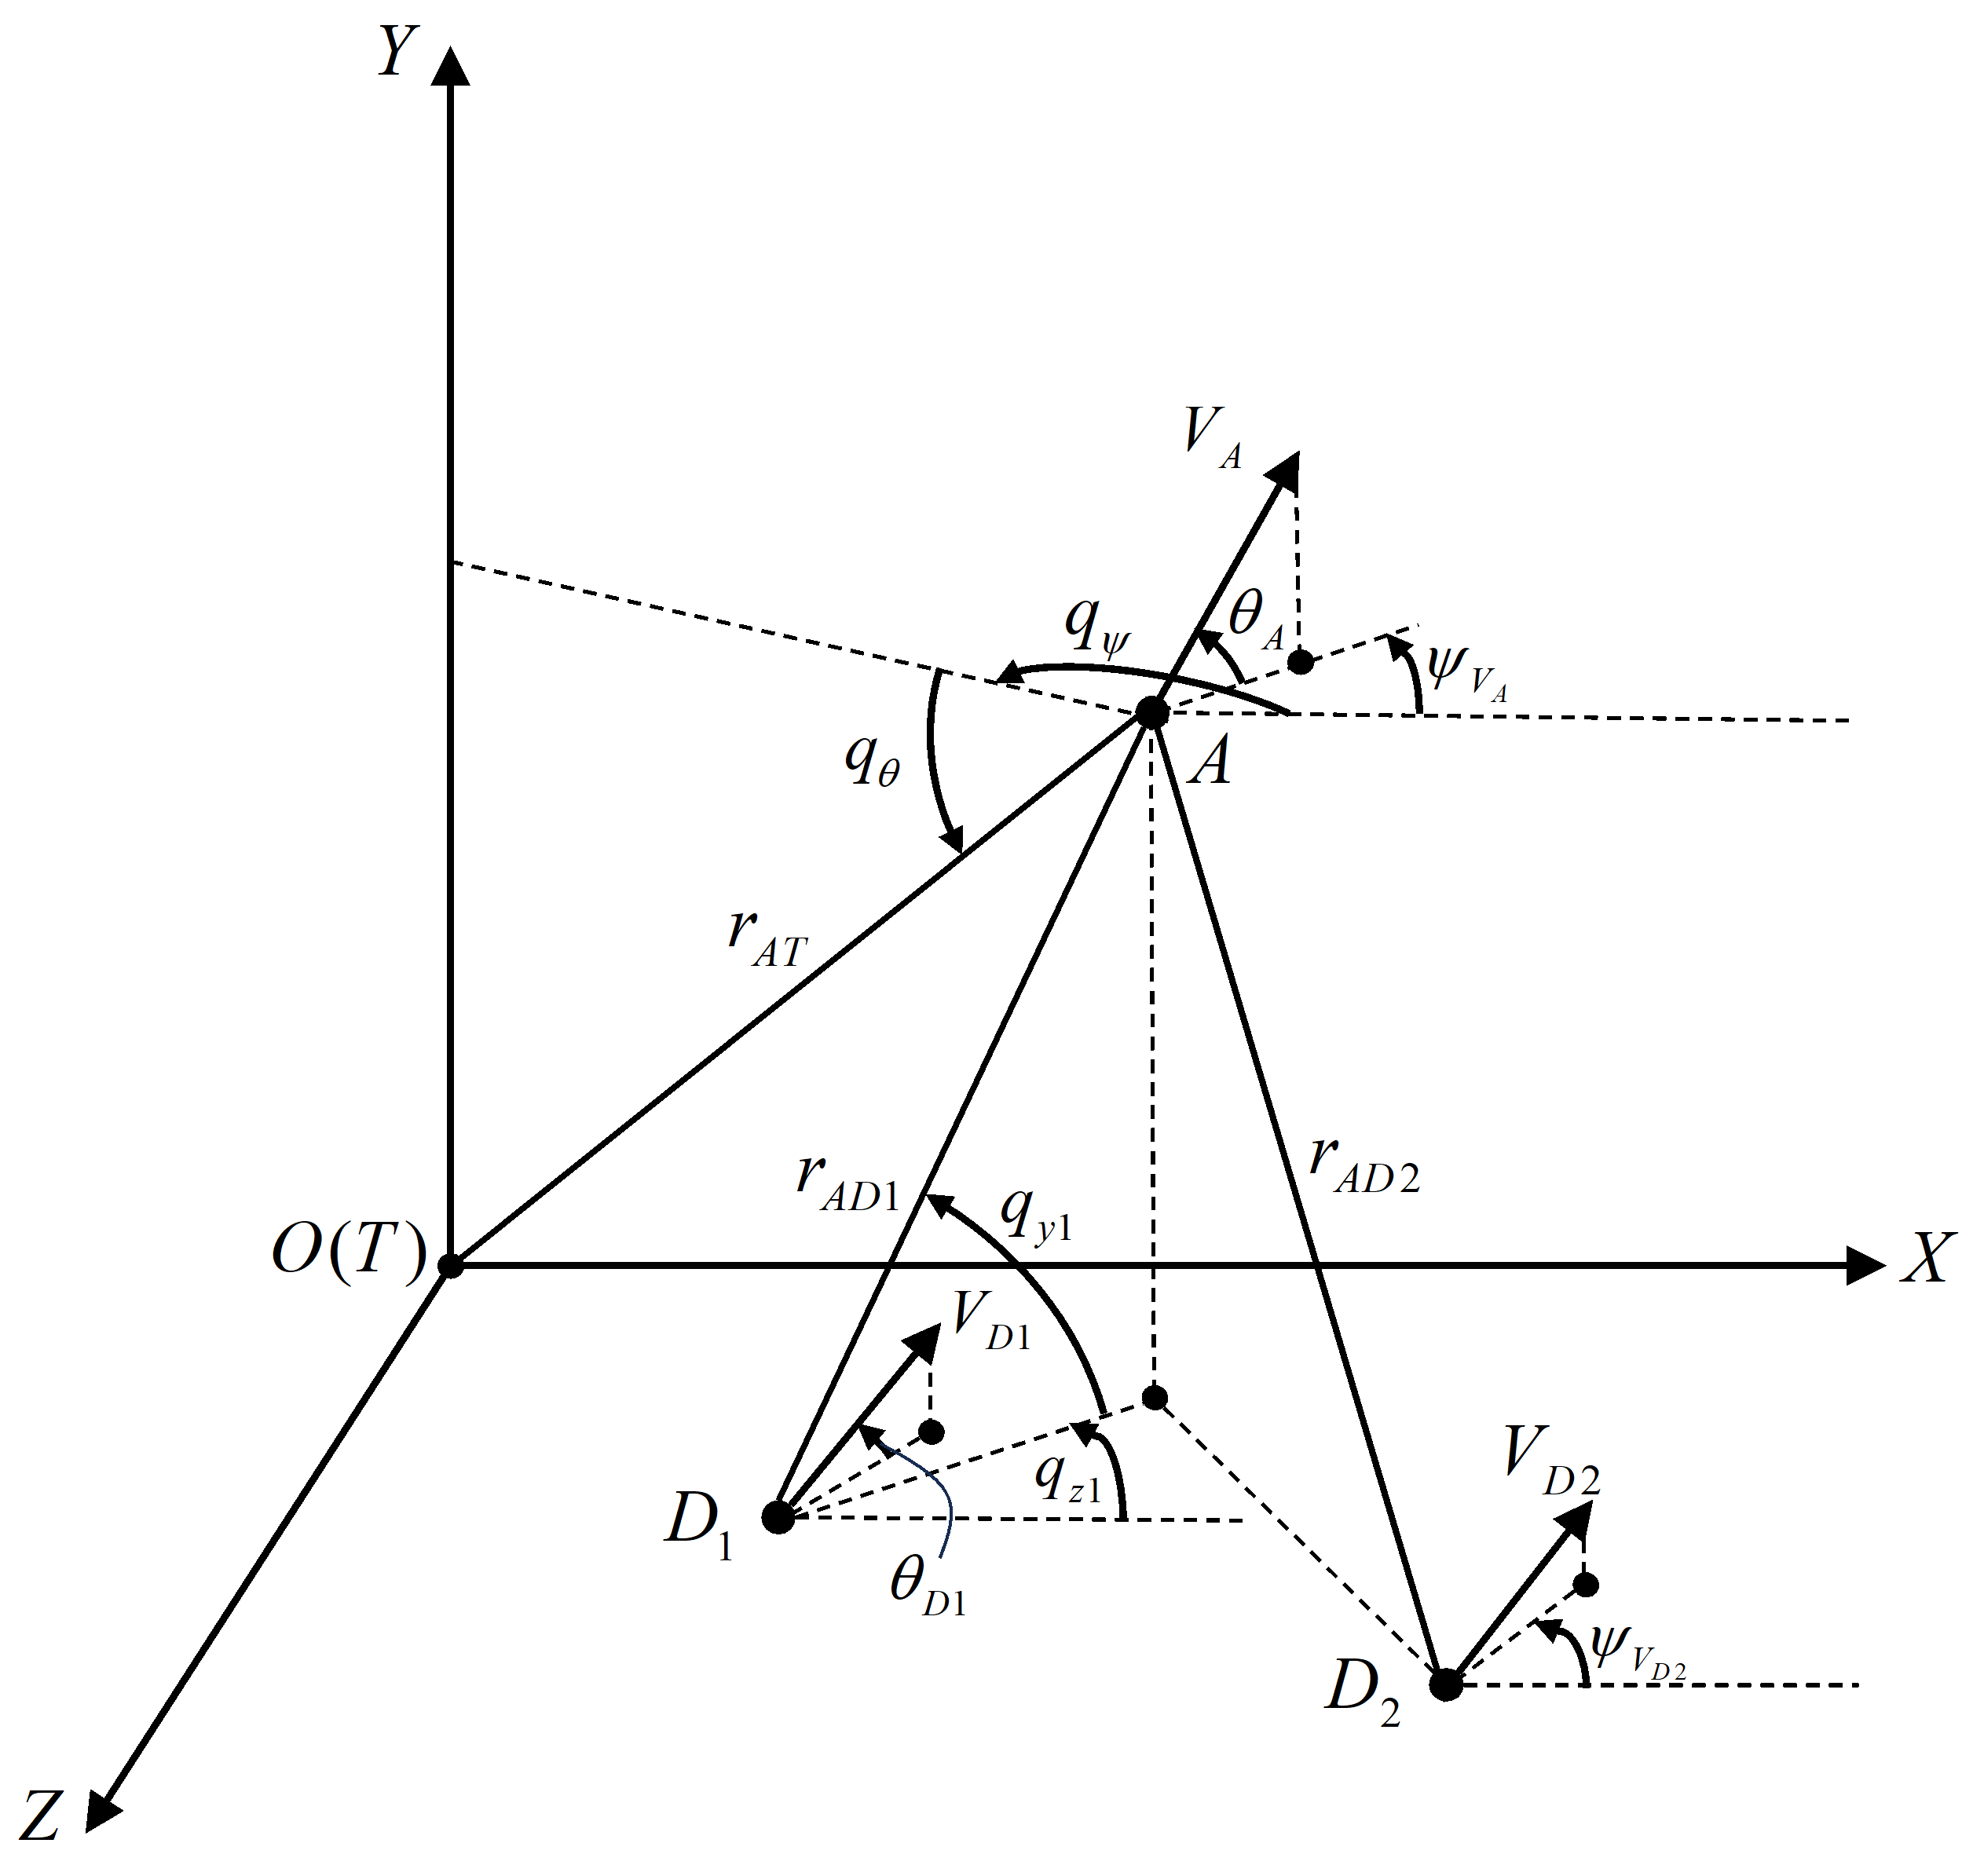
\includegraphics[width=0.585\linewidth]{fig01}
\caption{Four-body relative geometry of the evader, the target, NCV~1, and NCV~2.}
\label{fig:fourbody}
\end{figure}
The symbols for relative position and motion in Fig.~\ref{fig:fourbody} are listed in Table~\ref{tab:symbols}.

\begin{table}[!ht]
\centering
\caption{Symbols of relative position and motion in Fig.~\ref{fig:fourbody}.}
\label{tab:symbols}
\small
\begin{tabularx}{\linewidth}{lXX}
\toprule
Symbol & Meaning & Sign in Fig.~\ref{fig:fourbody} \\
\midrule
${r_{AT}},{r_{ADi}}$ & Ranges from the evader to the target and to the $i$th NCV & Positive, positive \\
${q_{yi}},{q_{zi}}$ & Elevation and azimuth LOS angles of the $i$th NCV & Positive, positive \\
${q_\theta },{q_\psi }$ & Elevation and azimuth LOS angles from the evader to the target & Negative, positive \\
${V_{Di}},{\theta _{Di}},{\psi _{{V_{Di}}}}$ & Speed, flight-path angle, and heading angle of the $i$th NCV & Positive, positive \\
${V_A},{\theta _A},{\psi _{{V_A}}}$ & Speed, flight-path angle, and heading angle of the evader & Positive, positive \\
\bottomrule
\end{tabularx}
\end{table}
\FloatBarrier
The relative-motion equations of NCVs ${D_1}$ and ${D_2}$ with respect to the evader $A$ are

\begin{equation}
\label{eq:1}
\left\{ {\begin{array}{*{20}{l}}
  \begin{aligned}
& {{\dot r}_{ADi}} =  - {V_{Di}}\left[ {\cos {\theta _{Di}}\cos {q_{yi}}\cos \left( {{q_{zi}} - {\psi _{{V_{Di}}}}} \right) + \sin {\theta _{Di}}\sin {q_{yi}}} \right] +  \\
& {\text{   }}{V_A}\left[ {\cos {\theta _A}\cos {q_{yi}}\cos \left( {{q_{zi}} - {\psi _{{V_A}}}} \right) + \sin {\theta _A}\sin {q_{yi}}} \right]
\end{aligned} \\
  \begin{aligned}
& {{\dot q}_{yi}}{r_{ADi}} = {V_{Di}}\left[ {\cos {\theta _{Di}}\sin {q_{yi}}\cos \left( {{q_{zi}} - {\psi _{{V_{Di}}}}} \right) - \sin {\theta _{Di}}\cos {q_{yi}}} \right] -  \\
& {V_A}\left[ {\cos {\theta _A}\sin {q_{yi}}\cos \left( {{q_{zi}} - {\psi _{{V_A}}}} \right) - \sin {\theta _A}\cos {q_{yi}}} \right]
\end{aligned} \\
  \begin{aligned}
& {{\dot q}_{zi}}{r_{ADi}}\cos {q_{yi}} = {V_{Di}}\cos {\theta _{Di}}\sin \left( {{q_{zi}} - {\psi _{{V_{Di}}}}} \right) -  \\
& {\text{           }}{V_A}\cos {\theta _A}\sin \left( {{q_{zi}} - {\psi _{{V_A}}}} \right)
\end{aligned}
\end{array}} \right.
\end{equation}
The relative-motion equations of the evader and the target are

\begin{equation}
\label{eq:2}
\left\{ {\begin{array}{*{20}{l}}
  {{{\dot r}_{AT}} =  - {V_A}\left[ {\sin {q_\theta }\sin {\theta _A} + \cos \left( {{q_\psi } - {\psi _{{V_A}}}} \right)\cos {q_\theta }\cos {\theta _A}} \right]} \\ 
  {{{\dot q}_\theta } = \frac{{{V_A}\left[ {\cos {\theta _A}\sin {q_\theta }\cos \left( {{q_\psi } - {\psi _{{V_A}}}} \right) - \sin {\theta _A}\cos {q_\theta }} \right]}}{{{r_{AT}}}}} \\ 
  {{{\dot q}_\psi } = \frac{{{V_A}\cos {\theta _A}\sin \left( {{q_\psi } - {\psi _{{V_A}}}} \right)}}{{{r_{AT}}\cos {q_\theta }}}} 
\end{array}} \right.
\end{equation}
The relative acceleration along the line of sight between each NCV and the evader follows from the kinematic relations:

\begin{equation}
\label{eq:3}
{\ddot r_{ADi}} = {r_{ADi}}\dot q_{yi}^2 + {r_{ADi}}\dot q_{zi}^2{\cos ^2}{q_{yi}} + {u_{ri}} - {v_{ri}}
\end{equation}
where ${u_{ri}}$ and ${v_{ri}}$ are the projections of the accelerations of the evader and the $i$th NCV onto the $x$ axis of the NCV--evader line-of-sight frame (denoted ${S_i}$). The positive $x$ axis points from the NCV toward the evader.

The relative acceleration along the line of sight between the target and the evader is

\begin{equation}
\label{eq:4}
{\ddot r_{AT}} = {r_{AT}}\dot q_\theta ^2 + {r_{AT}}\dot q_\psi ^2{\cos ^2}{q_\theta } + {u_{rT}}
\end{equation}
where ${u_{rT}}$ is the projection of the evader acceleration onto the $x$ axis of the target--evader line-of-sight frame (denoted ${S_T}$). The positive $x$ axis points from the target toward the evader.

For each vehicle, the three-dimensional kinematic equations are

\begin{equation}
\label{eq:5}
\left\{ {\begin{array}{*{20}{l}}
  {{{\dot x}_j} = {V_j}\cos {\theta _j}\cos {\psi _{{V_j}}}} \\ 
  {{{\dot y}_j} = {V_j}\sin {\theta _j}} \\ 
  {{{\dot z}_j} =  - {V_j}\cos {\theta _j}\sin {\psi _{{V_j}}}} \\ 
  {{{\dot \theta }_j} = \frac{{{a_{yj}}}}{{{V_j}}}} \\ 
  {{{\dot \psi }_j} =  - \frac{{{a_{zj}}}}{{{V_j}\cos {\theta _j}}}} 
\end{array},j = A,{D_1},{D_2}} \right.
\end{equation}
where $({x_j},{y_j},{z_j})$ are the vehicle coordinates in the Earth-fixed frame. Both ${a_{yj}}$ and ${a_{zj}}$ are perpendicular to the velocity vector and denote the normal acceleration components along the $y$ and $z$ axes of the flight-path frame. The former lies in the vertical plane containing the velocity vector, and the latter lies in the horizontal $xOz$ plane of the Earth-fixed frame.

From the line-of-sight relative-acceleration relations, the projections ${u_{ri}}$ and ${v_{ri}}$ of the evader and the $i$th NCV accelerations onto the $x$ axis of the line-of-sight frame ${S_i}$ are related to the normal accelerations ${a_{yA}}$, ${a_{zA}}$ and ${a_{yDi}}$, ${a_{zDi}}$ by a coordinate transformation. Let ${\mathbf{L}}({q_{yi}},{q_{zi}})$ be the transformation from the Earth-fixed frame to the line-of-sight frame ${S_i}$, and let ${\mathbf{L}}(\theta ,{\psi _V})$ be the transformation from the Earth-fixed frame to the flight-path frame. The two projections are then

\begin{equation}
\label{eq:6}
{u_{ri}} = \left[ {\begin{array}{*{20}{c}}
  1&0&0 
\end{array}} \right]{\mathbf{L}}({q_{yi}},{q_{zi}}){{\mathbf{L}}^{ - 1}}({\theta _A},{\psi _{{V_A}}})\left[ {\begin{array}{*{20}{c}}
  0 \\ 
  {{a_{yA}}} \\ 
  {{a_{zA}}} 
\end{array}} \right]
\end{equation}
\begin{equation}
\label{eq:7}
{v_{ri}} = \left[ {\begin{array}{*{20}{c}}
  1&0&0 
\end{array}} \right]{\mathbf{L}}({q_{yi}},{q_{zi}}){{\mathbf{L}}^{ - 1}}({\theta _{Di}},{\psi _{{V_{Di}}}})\left[ {\begin{array}{*{20}{c}}
  0 \\ 
  {{a_{yDi}}} \\ 
  {{a_{zDi}}} 
\end{array}} \right]
\end{equation}
The explicit form of the transformation matrices follows the standard definition of three-dimensional coordinate transformations and is omitted here. Likewise, let ${\mathbf{L}}( - {q_\theta },{q_\psi } - \pi )$ be the transformation from the Earth-fixed frame to the line-of-sight frame ${S_T}$, where the line-of-sight angles are the elevation and azimuth corresponding to the positive $x$ axis of ${S_T}$ (from the target toward the evader). The projection of the evader acceleration onto the $x$ axis of ${S_T}$ is then

\begin{equation}
\label{eq:8}
{u_{rT}} = \left[ {\begin{array}{*{20}{c}}
  1&0&0 
\end{array}} \right]{\mathbf{L}}( - {q_\theta },{q_\psi } - \pi ){{\mathbf{L}}^{ - 1}}({\theta _A},{\psi _{{V_A}}})\left[ {\begin{array}{*{20}{c}}
  0 \\ 
  {{a_{yA}}} \\ 
  {{a_{zA}}} 
\end{array}} \right]
\end{equation}
\begin{assumption}[NCV guidance law and performance]
\label{asm:ncv}
The guidance laws and performance parameters of the two NCVs are known to the evader. Both NCVs employ the classical proportional-navigation (PN) guidance law~\cite{murtaugh1966}, with acceleration commands
\begin{equation}
\label{eq:9}
\left[ {\begin{array}{*{20}{c}}
  {{a_{yDi}}} \\ 
  {{a_{zDi}}} 
\end{array}} \right] = \left[ {\begin{array}{*{20}{c}}
  {{K_{Di}}{V_{Di}}{{\dot q}_{yi}}} \\ 
  { - {K_{Di}}{V_{Di}}{{\dot q}_{zi}}\cos {\theta _{Di}}} 
\end{array}} \right]
\end{equation}
where ${K_{Di}}$ is the proportional-navigation gain of the $i$th NCV. The two NCVs have identical performance, that is, ${K_{{D_1}}} = {K_{{D_2}}} = {K_D}$ and ${V_{{D_1}}} = {V_{{D_2}}} = {V_D}$, and both ${K_D}$ and ${V_D}$ remain constant during the engagement.
\end{assumption}
The desired evasion distances of the two NCVs are taken to be equal, that is, $d_1^* = d_2^* = d^*$.
\subsection{Linearized state-space model}
Substituting \eqref{eq:6}, \eqref{eq:7}, and the associated transformation matrices into \eqref{eq:3} yields

\begin{equation}
\label{eq:10}
\begin{gathered}
  {{\ddot r}_{ADi}} = {r_{ADi}}\left( {\dot q_{yi}^2 + \dot q_{zi}^2{{\cos }^2}{q_{yi}}} \right) - \cos {q_{yi}}\sin \left( {{q_{zi}} - {\psi _{{V_A}}}} \right){a_{zA}} +  \\ 
  {a_{yA}}\left[ { - \cos {q_{yi}}\sin {\theta _A}\cos \left( {{q_{zi}} - {\psi _{{V_A}}}} \right) + \sin {q_{yi}}\cos {\theta _A}} \right] -  \\ 
  {a_{yDi}}\left[ { - \cos {q_{yi}}\sin {\theta _{Di}}\cos \left( {{q_{zi}} - {\psi _{{V_{Di}}}}} \right) + \sin {q_{yi}}\cos {\theta _{Di}}} \right] +  \\ 
  \cos {q_{yi}}\sin \left( {{q_{zi}} - {\psi _{{V_{Di}}}}} \right){a_{zDi}} \\ 
\end{gathered}
\end{equation}
Likewise, substituting \eqref{eq:8} and the associated transformation matrix into \eqref{eq:4} yields

\begin{equation}
\label{eq:11}
\begin{gathered}
  {{\ddot r}_{AT}} = {r_{AT}}\left( {\dot q_\theta ^2 + \dot q_\psi ^2{{\cos }^2}{q_\theta }} \right) + \left[ {\sin {\theta _A}\cos {q_\theta }\cos \left( {{q_\psi } - {\psi _{{V_A}}}} \right) - \cos {\theta _A}\sin {q_\theta }} \right]{a_{yA}} +  \\ 
  \cos {q_\theta }\sin \left( {{q_\psi } - {\psi _{{V_A}}}} \right){a_{zA}} \\ 
\end{gathered}
\end{equation}
Define the state ${x_i} = {\left[ {\begin{array}{*{20}{c}}
  {{r_{ADi}}}&{{{\dot r}_{ADi}}} 
\end{array}} \right]^T}$ and the control\[{u_A} = {\left[ {\begin{array}{*{20}{c}}
  {{a_{yA}}}&{{a_{zA}}} 
\end{array}} \right]^T}\]. The state-space equation of the interaction between the evader and the $i$th NCV is then

\begin{equation}
\label{eq:12}
\mathop {{x_i}}\limits^. (t) = {{\mathbf{A}}_i}{x_i}(t) + {{\mathbf{B}}_i}{u_A}(t) + {{\mathbf{C}}_i}
\end{equation}
where
\[{{\mathbf{A}}_i} = \left[ {\begin{array}{*{20}{c}}
  0&1 \\ 
  {\dot q_{yi}^2 + \dot q_{zi}^2{{\cos }^2}{q_{yi}}}&0 
\end{array}} \right],\ {{\mathbf{B}}_i} = \left[ {\begin{array}{*{20}{c}}
  0&0 \\ 
  {{B_{1,i}}}&{{B_{2,i}}} 
\end{array}} \right],\ {{\mathbf{C}}_i} = \left[ {\begin{array}{*{20}{c}}
  0 \\ 
  {{C_{1i}}} 
\end{array}} \right]\]
with

\begin{equation}
\label{eq:13}
\left\{ {\begin{array}{*{20}{l}}
  {{B_{1,i}} = \sin {q_{yi}}\cos {\theta _A} - \cos {q_{yi}}\sin {\theta _A}\cos \left( {{q_{zi}} - {\psi _{{V_A}}}} \right)} \\ 
  {{B_{2,i}} =  - \cos {q_{yi}}\sin \left( {{q_{zi}} - {\psi _{{V_A}}}} \right)} \\ 
  {{C_{1i}} = \cos {q_{yi}}\sin \left( {{q_{zi}} - {\psi _{{V_{Di}}}}} \right){a_{zDi}} + [\cos {q_{yi}}\sin {\theta _{Di}}\cos \left( {{q_{zi}} - {\psi _{{V_{Di}}}}} \right) - \sin {q_{yi}}\cos {\theta _{Di}}]{a_{yDi}}} 
\end{array}} \right.
\end{equation}
Define the state ${x_{AT}} = {\left[ {\begin{array}{*{20}{c}}
  {{r_{AT}}}&{{{\dot r}_{AT}}} 
\end{array}} \right]^T}$. The relative state-space equation of the evader and the target is then

\begin{equation}
\label{eq:14}
{\dot x_{AT}}(t) = {{\mathbf{A}}_T}{x_{AT}}(t) + {{\mathbf{B}}_T}{u_A}(t)
\end{equation}
where
\[{{\mathbf{A}}_T} = \left[ {\begin{array}{*{20}{c}}
  0&1 \\ 
  {\dot q_\theta ^2 + \dot q_\psi ^2{{\cos }^2}{q_\theta }}&0 
\end{array}} \right],\ {{\mathbf{B}}_T} = \left[ {\begin{array}{*{20}{c}}
  0&0 \\ 
  {{B_{1,T}}}&{{B_{2,T}}} 
\end{array}} \right]\]
with

\begin{equation}
\label{eq:15}
\left\{
\begin{aligned}
& {B_{1,T}} = \sin {\theta _A}\cos {q_\theta }\cos \left( {{q_\psi } - {\psi _{{V_A}}}} \right) - \cos {\theta _A}\sin {q_\theta } \\
& {B_{2,T}} = \cos {q_\theta }\sin \left( {{q_\psi } - {\psi _{{V_A}}}} \right)
\end{aligned}
\right.
\end{equation}
\begin{remark}
The system \eqref{eq:12}--\eqref{eq:15} is linear and time-varying. To obtain an analytical guidance command, each matrix is frozen at its current value and treated as constant in the prediction of a given guidance cycle, and is recomputed from the updated state in the next cycle. This quasi-frozen-coefficient treatment also provides the basis for the online parameter identification in Section~4.
\end{remark}
\begin{assumption}[Measurement conditions]
\label{asm:meas-noise}
In practice, the matrix elements in \eqref{eq:12}--\eqref{eq:15} are obtained from the onboard seeker and IMU, rather than from noise-free ideal kinematics. Two classes of measurement noise are considered. The first is angular: the measured line-of-sight angles, line-of-sight rates, and vehicle flight-path and heading angles are each corrupted by zero-mean Gaussian white noise:
\begin{equation}
\label{eq:16}
\begin{gathered}
  \tilde{q}_{\alpha} = {q_{\alpha}} + {\nu _{q,\alpha }},\quad {\nu _{q,\alpha }}\sim \mathcal{N}(0,\sigma _q^2), \hfill \\
  \tildedot{q}_{\alpha} = \dot{q}_{\alpha} + {\nu _{\dot q,\alpha }},\quad {\nu _{\dot q,\alpha }}\sim \mathcal{N}(0,\sigma _{\dot q}^2), \hfill \\
  \tilde{\theta}_{j} = {\theta _{j}} + {\nu _{\theta ,j}},\quad {\nu _{\theta ,j}}\sim \mathcal{N}(0,\sigma _\theta ^2), \hfill \\
  \tilde{\psi}_{V_{j}} = {\psi _{V_{j}}} + {\nu _{\psi ,j}},\quad {\nu _{\psi ,j}}\sim \mathcal{N}(0,\sigma _\psi ^2), \hfill \\ 
\end{gathered}
\end{equation}
where $\alpha  \in \left\{ {{y_i},{z_i},\theta ,\psi } \right\}$ indexes the line-of-sight channels to the $i$th NCV and to the target, and $j \in \left\{ {A,{D_1},{D_2}} \right\}$. The second class is range: the relative range and range rate of each channel are likewise corrupted by zero-mean Gaussian white noise

\begin{equation}
\label{eq:16b}
\tilde{r}_{c} = {r_c} + {\nu _{r,c}},\quad {\nu _{r,c}}\sim \mathcal{N}(0,\sigma _r^2),\quad
\tildedot{r}_{c} = {\dot r_c} + {\nu _{\dot r,c}},\quad {\nu _{\dot r,c}}\sim \mathcal{N}(0,\sigma _{\dot r}^2)
\end{equation}
where $c \in \left\{ {1,2,T} \right\}$ corresponds to the three range channels ${r_{AD1}}$, ${r_{AD2}}$, and ${r_{AT}}$. A radar seeker measures range from echo delay and range rate from coherent Doppler. Their relative accuracy is limited mainly by signal bandwidth and coherent integration time, whereas angular measurements are limited by beamwidth, target glint, and coupling with vehicle motion, and are typically one to two orders of magnitude less accurate~\cite{skolnik2008}. Accordingly, ${\sigma _r}$ and ${\sigma _{\dot r}}$ are taken to be small; their numerical values are given in Section~6.1. In addition, the relative acceleration $\ddot{r}$ cannot be measured directly and must be estimated online from the noisy $\tilde{r}$ and $\tildedot{r}$. The normal accelerations ${a_{yA}}$ and ${a_{zA}}$ actually applied by the evader are known onboard.

The matrix elements in \eqref{eq:13} and \eqref{eq:15} are nonlinear functions of four angular measurements. Substituting the measurements directly produces biased and mutually correlated errors that enter the acceleration command through the guidance law. Range measurements are more accurate, and their errors can be further suppressed by filtering. Section~4 therefore builds an online identification framework that recovers the matrix elements from relative-range kinematics, without relying on the noise-sensitive analytical expressions \eqref{eq:12}--\eqref{eq:15}.
\end{assumption}

\subsection{Optimal-problem formulation}
To reduce the system order and simplify the solution, the zero-effort miss (ZEM) $z(t)$ is introduced. The ZEM of the evader relative to the $i$th NCV is defined as

\begin{equation}
\label{eq:17}
{z_i}(t) = \left[ {\begin{array}{*{20}{c}}
  1&0 
\end{array}} \right]\Omega \left( {{t_{fi}},t} \right){x_i}(t)
\end{equation}
where the state-transition matrix is

\begin{equation}
\label{eq:18}
\Omega \left( {{t_{fi}},t} \right) = {e^{{A_i}\left( {{t_{fi}} - t} \right)}} = \left[ {\begin{array}{*{20}{c}}
  {\cosh ({{\dot Q}_i}{t_{{\text{go,i}}}})}&{\frac{{\sinh ({{\dot Q}_i}{t_{{\text{go,i}}}})}}{{{{\dot Q}_i}}}} \\ 
  {{{\dot Q}_i}\sinh ({{\dot Q}_i}{t_{{\text{go,i}}}})}&{\cosh ({{\dot Q}_i}{t_{{\text{go,i}}}})} 
\end{array}} \right]
\end{equation}
with ${\dot Q_i} = \sqrt {\dot q_{yi}^2 + \dot q_{zi}^2{{\cos }^2}{q_{yi}}} $ the composite line-of-sight rate and ${t_{go,i}} = {t_{fi}} - t$ the time-to-go. Using $\dot \Omega \left( {{t_{fi}},t} \right) =  - \Omega \left( {{t_{fi}},t} \right){A_i}$ and differentiating \eqref{eq:17} gives

\begin{equation}
\label{eq:19}
{\dot z_i}(t) = {\varphi _i}(t)b_i^T{u_A}(t) - {\varphi _i}(t){v_{ri}}
\end{equation}
where

\begin{equation}
\label{eq:20}
\left\{
\begin{aligned}
& {\varphi _i}(t) = \frac{{{e^{{{\dot Q}_i}{t_{go,i}}}} - {e^{ - {{\dot Q}_i}{t_{go,i}}}}}}{{2{{\dot Q}_i}}} \\
& {b_i} = {\left[ {\begin{array}{*{20}{c}}
  {{B_{1,i}}}&{{B_{2,i}}}
\end{array}} \right]^T}
\end{aligned}
\right.
\end{equation}
The derivative of the evader--target ZEM is obtained in the same way:

\begin{equation}
\label{eq:21}
{\dot z_T}(t) = {\varphi _T}(t)b_T^T{u_A}(t)
\end{equation}
where

\begin{equation}
\label{eq:22}
\left\{
\begin{aligned}
& {\varphi _T}(t) = \frac{{{e^{{{\dot Q}_T}{t_{go,T}}}} - {e^{ - {{\dot Q}_T}{t_{go,T}}}}}}{{2{{\dot Q}_T}}} \\
& {b_T} = {\left[ {\begin{array}{*{20}{c}}
  {{B_{1,T}}}&{{B_{2,T}}}
\end{array}} \right]^T}
\end{aligned}
\right.
\end{equation}
with ${\dot Q_T} = \sqrt {\dot q_\theta ^2 + \dot q_\psi ^2{{\cos }^2}{q_\theta }} $ and ${t_{go,T}} = {t_{fT}} - t$.

The objective of the intelligent evasion algorithm is to evade both NCVs successfully, minimize the maneuver energy, and avoid excessive maneuvering that would impair subsequent target arrival. The following quadratic performance index is therefore constructed:

\begin{equation}
\label{eq:23}
\mathop {\min }\limits_{{u_A}} J = \sum\nolimits_{i = 1}^2 {\frac{{{w_i}}}{2}{{\left[ {z_i\left( {{t_{fi}}} \right) - d_i^*} \right]}^2}}  + \frac{{{w_E}}}{2}\int_{{t_0}}^{{t_f}} {u_A^T{u_A}d\tau {\text{ + }}\frac{{{w_T}}}{2}z_T^2\left( {{t_{fT}}} \right)}
\end{equation}
where ${w_i} > 0$ is the weight on the evasion ZEM, ${w_E} > 0$ is the control-energy weight, ${w_T} > 0$ is the weight on the target-arrival ZEM, and $d_i^*$ is the desired evasion distance from the $i$th NCV, usually set slightly larger than the NCV lethal radius. ${t_f} = \max ({t_{f1}},{t_{f2}})$ is the terminal time of the overall evasion. To balance the two NCVs, set ${w_1} + {w_2} = w$ with $w$ a positive constant, and let ${w_1}$ and ${w_2}$ satisfy

\begin{equation}
\label{eq:24}
\left\{
\begin{aligned}
& {w_1} = w \cdot \frac{1}{{1 + {e^{ - \gamma }}}} \\
& {w_2} = w - {w_1} = w \cdot \frac{{{e^{ - \gamma }}}}{{1 + {e^{ - \gamma }}}}
\end{aligned}
\right.
\end{equation}
\begin{problem}[Integrated optimal evasion and guidance]
\label{prb:integrated}
Consider the dual-NCV proportional-navigation engagement in \cref{asm:ncv}. Taking the evader normal acceleration ${u_A} = {[{a_{yA}},{a_{zA}}]^T}$ as the control, and subject to the three-dimensional four-body kinematics \eqref{eq:1}--\eqref{eq:5} and the state-space equations \eqref{eq:12} ($i = 1,2$) and \eqref{eq:14}, together with the command-magnitude limit set by the maximum normal load factor available to the evader, find the optimal control $u_A^*(t)$ that minimizes the performance index \eqref{eq:23} expressed by the ZEMs \eqref{eq:17} and \eqref{eq:21}. That is, drive the evasion ZEM toward the desired evasion distance $d^*$ at the engagement instants ${t_{f1}}$ and ${t_{f2}}$ of the two NCVs, drive the target-arrival ZEM toward zero at ${t_{fT}}$, and minimize the control energy over the whole flight, with the two evasion weights allocated by \eqref{eq:24}.
\end{problem}

The problem above places evasion of both NCVs, arrival at the target, and control effort under the same optimality condition, rather than treating them by hierarchical decoupling. The integrated guidance law, the guidance-parameter optimization, and the online parameter identification in the remainder of the paper are all developed around its solution.

Solving \cref{prb:integrated} presents three difficulties.

First, the three tasks are coupled through the same control and the problem is not separable. The control ${u_A}$ enters the three relative channels simultaneously through the projection coefficients ${b_1}$, ${b_2}$, and ${b_T}$, which vary with the line-of-sight geometry and may change sign. A maneuver that increases the terminal separation from one NCV may reduce the separation from the other and change the ZEM of the target-arrival channel. The three terminal times ${t_{f1}}$, ${t_{f2}}$, and ${t_{fT}}$ differ, and the indicator functions further partition the problem in time. Consequently, \cref{prb:integrated} neither reduces to two independent single-NCV evasion subproblems nor is readily solved by online numerical optimization within the limited time-to-go of the terminal phase. Section~3 therefore applies the maximum principle together with the ZEM order reduction, and reduces the coupling to a $3 \times 3$ linear system, which yields a closed-loop analytical guidance command.

Second, the weights in the performance index \eqref{eq:23} cannot be fixed a priori. The evasion-weight allocation coefficient $\gamma$ and the relative magnitudes of ${w_T}$ and ${w_E}$ determine the trade-off among evasion, arrival, and energy. Their optimal values depend on the engagement geometry, the time-to-go, and the available load-factor margin. Biasing the weights too far toward evasion keeps the command near the load-factor limit for a long time and removes the subsequent arrival capability, whereas biasing them too far toward arrival leaves insufficient evasion margin. Weight selection is therefore itself a nonlinear optimization problem along the trajectory. Section~5 uses optimal expert trajectories generated by shooting for actor pre-training, replay-buffer pre-filling, and a decaying behavior-cloning constraint during TD3 fine-tuning, after which the trained actor produces the weights online.

Third, the parameters required by the analytical guidance law are not directly available under realistic measurements. The coefficients ${b_i}$ and ${b_T}$, the composite rates ${\dot Q_i}$ and ${\dot Q_T}$, and the NCV maneuver projection ${v_{ri}}$ are nonlinear functions of the line-of-sight angles, line-of-sight rates, and flight-path angles. Substituting noisy measurements into the analytical expressions \eqref{eq:12}--\eqref{eq:15} as in \cref{asm:meas-noise} produces biased and mutually correlated errors that enter the guidance command directly, and the relative acceleration cannot be measured directly either. Section~4 therefore constructs a recursive least-squares identifier with sparse regularization and a forgetting factor, which recovers these parameters online from relative-range kinematics and closes the loop with the guidance law.
